\section{Turbulence II}

Last time we saw some exact results for Stokes' flow (fluid flow at low Reynolds number) in the presence of odd viscosity. Usually, at higher Reynolds number, the calculations become less and less analytically tractable. But there are some aspects that become accessible to study via a statistical mechanics lens - we discuss them today.

\subsection{Review}
We looked at $\log E(k)$, the logartihm of the power spectrum:

\begin{center}
    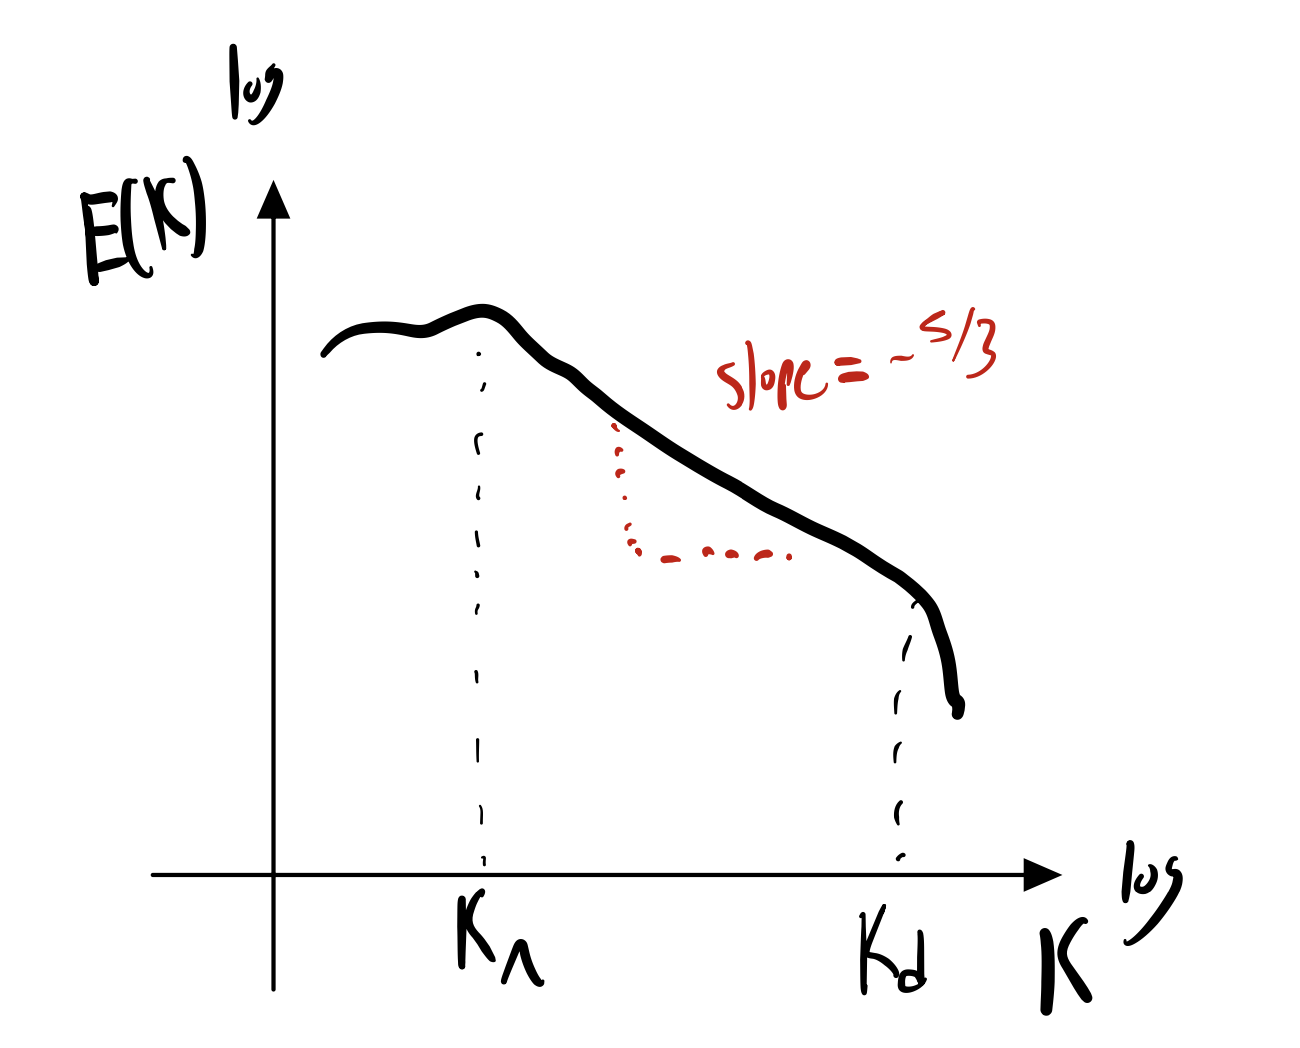
\includegraphics[scale=0.35]{Lectures/Images/lec11-spectrum.png}
\end{center}
where in the inertial range $k_\lambda \leq k \leq k_d$ (where the dissipative scale $k_d$ is set by when $\text{Re} = \frac{UL}{\nu} \sim 1$). Here, we have:
\begin{equation}
    E(k) \sim \e^{2/3}k^{-5/3}
\end{equation}
and the Navier-Stokes equations reduce to:
\begin{equation}
    \text{Re}(\p_t \v{v} + \v{v} \cdot \nabla \v{v}) = \nabla p + v \nabla^2\v{v}
\end{equation}
Where a key assumption in the derivation was that the energy flux was constant:
\begin{equation}
    \Pi_l \sim \frac{v_l^2}{\tau_l} \sim \frac{v_l^3}{l} = \text{const.} = \e
\end{equation}

\subsection{Estimating the dissipative scale}
Recall back to a particle falling in a viscous medium - the power dissipated is given by $P = \v{F} \cdot \v{v} \propto \eta v(v) = \eta v^2$. In continuum theory, we promote this to:
\begin{equation}
    P \propto \eta_{ijkl}v_{ij}v_{kl}
\end{equation}
with $v_{ij} = \p_i v_j$. 

So, let us estimate:
\begin{equation}
    P \sim \nu(\p_i v_j)^2
\end{equation}
The first scale at which dissipation starts to become non-negligible is at $k = k_d$. So, estimating the power at this point:
\begin{equation}
    P \sim \nu \left(\frac{v_d}{\eta_d}\right)^2
\end{equation}
with $\eta_d \sim \frac{1}{k_d}$ - this ensures that:
\begin{equation}
    \text{Re} \sim \frac{v_d\eta_d}{\nu} \sim 1.
\end{equation}
Physically, we can imagine that $v_d$ is the smallest scale speed and $\eta_d$ is the length corresponding to the smallest eddy size. Now, we make the assumption that all of the energy injected into the system at $k = k_\Lambda$ is dissipated at $k = k_d$. So, our estimate of the energy flux is:
\begin{equation}
    \e \sim \nu \left(\frac{v_d}{\eta_d}\right)^2
\end{equation}
Now, we can say that, since the effective Reynolds is $\text{Re} \sim 1$ at $k_d$:
\begin{equation}
    v_d \sim \frac{\nu}{\eta_d}
\end{equation}
Now, we can say:
\begin{equation}
    \eta \sim \nu \left(\frac{\frac{\nu}{\eta_d}}{\eta_d}\right)^2 = \frac{\nu^3}{\eta_d^4}
\end{equation}
Thus isolating for $\eta_d$ and thus $k_d$:
\begin{equation}
    \eta_d \sim \left(\frac{\nu^3}{\e}\right)^{1/4} \implies k_d \sim \left(\frac{\e}{\nu^3}\right)^{1/4}
\end{equation}
Now, let us write $\e = \frac{U^3}{L}$ (where $U$ is the macroscopic speed scale in which we inject energy), so:
\begin{equation}
    \eta_d \sim \left(L\frac{\nu^3}{U^3}\right)^{1/4}
\end{equation}
Now, by multiplying this by one, we can write this in terms of the original Reynolds number $\text{Re} = \frac{UL}{\nu}$:
\begin{equation}
    \eta_d \sim \left(\frac{\nu^3}{U^3L^3}L^4\right)^{1/4} \sim \text{Re}^{-3/4}L
\end{equation}
hence we have the conclusion:
\begin{equation}
   \boxed{\frac{\eta_d}{L} \sim \frac{1}{\text{Re}^{3/4}}}
\end{equation}
where $\text{Re}$ is the Reynolds number at injection.

Let's now plug in the Reynolds number for a given experimental setup. We consider an experimental setup where we have fluid of Reynolds number $\text{Re} \sim 10^3$ flowing through a grid of grid size $l \sim \text{1}\si{cm}$:

\begin{center}
    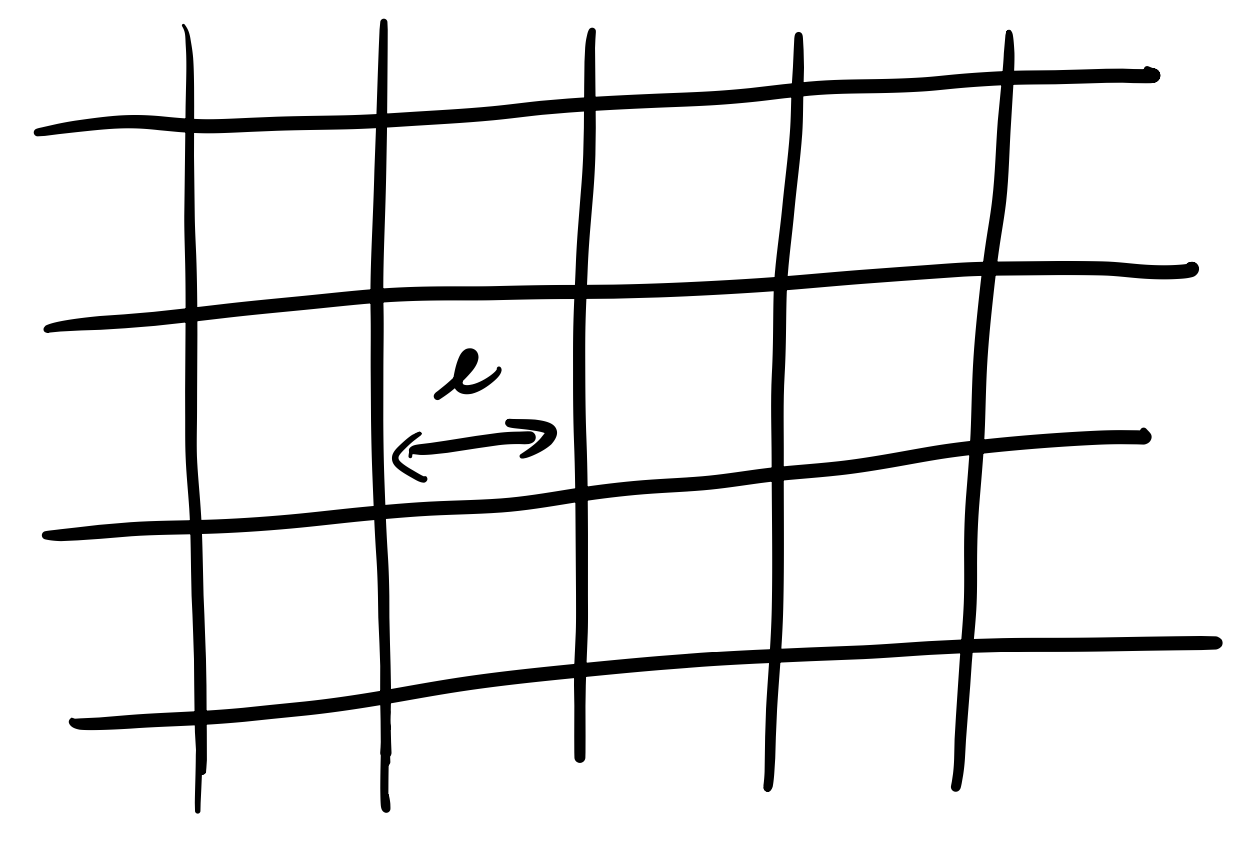
\includegraphics[scale=0.35]{Lectures/Images/lec13-lattice.png}
\end{center}

Which yields:
\begin{equation}
    \eta_d \sim 0.06\si{mm}
\end{equation}
We can see from this simple calculation how this scaling is quite unfavourable for experimentalists - we have sublinear scaling in the Reynolds number. To span many decades is quite difficult.

\subsection{Enstrophy and the Zeroth Law of Turbulence}
We wish to evaluate the power/rate at which we lose energy due to viscosity, $\pd{E}{t}$. We start with the change in kinetic energy of the system, and rewrite it using Navier-Stokes:
\begin{equation}
    \frac{1}{2}\rho_0\frac{\partial(\v{u}^2)}{\partial t} = \rho_0 \v{u}\cdot \dpd{\v{u}}{t} = \rho_0 \v{u}\cdot\left(-\v{u}\cdot\nabla\v{u} - \frac{\nabla p}{\rho_0} + \nu\nabla^2\v{u}\right)
\end{equation}
Now, we rewrite:
\begin{equation}
    \v{u} \cdot \nabla^2 \v{u} = -\v{u} \cdot (\nabla \times (\nabla \times \v{u})) = -\v{u} \cdot (\nabla \times \gv{\omega})
\end{equation}
where we define $\gv{\omega} = \nabla \times \v{u}$ the vorticity, and in the above vector field identity we have assumed incompressibility $\nabla \cdot \v{u} = 0$. We can further rewrite:
\begin{equation}
    \v{u} \cdot \nabla^2\v{u} = \nabla\cdot(\v{u} \times \gv{\omega}) - \gv{\omega}^2
\end{equation}
Our expression for the kinetic energy loss becomes (again using $\nabla \cdot \v{u} = 0$ where necessary):
\begin{equation}
    \frac{1}{2}\rho_0\frac{\partial(\v{u}^2)}{\partial t} = -\rho_0 \v{u} \cdot \nabla\left(\frac{u^2}{2}\right) - \nabla \cdot (p\v{u} - \rho_0 \nu(\v{u} \times \gv{\omega})) - \rho_0 \nu\gv{\omega}^2
\end{equation}
Hence:
\begin{equation}
    \pd{E}{t} = -\nabla\cdot\underbrace{\left[\left(\rho_0\frac{\v{v}^2}{2} + p\right)\v{u} - \rho_0\nu \v{u} \times \gv{\omega}\right]}_{\text{flux}} - \underbrace{\rho_0 \nu \gv{\omega}^2}_{\text{source/sink}}
\end{equation}
If we assume that $\v{u} = \v{0}$ sufficiently quickly at the boundaries of the system, or we have periodic boundary conditions, we may drop the flux term, and we thus only study:
\begin{equation}
    \boxed{\dpd{E}{t} = -\rho_0 \nu\gv{\omega}^2}
\end{equation}
so the energy loss is proportional to the vorticity squared.

The volume version of this is:
\begin{equation}
    \dpd{}{t}\iiint E dV = -\oiint \v{F} \cdot \hat{\v{n}}dS - \rho_0v \iiint \gv{\omega}^2 dV
\end{equation}

In $d$-dimensions, we can define the enstropy per unit volume (area) as:
\begin{equation}
    \Omega = \frac{\text{Enstrophy}}{L^d} = \frac{1}{2}\avg{\gv{\omega}^2}
\end{equation}
Wherein:
\begin{equation}
    \dpd{\avg{E}}{t} = -\rho_0 \nu \avg{\gv{\omega^2}}
\end{equation}
Now, the energy flux/loss we have also taken to be $\e(\nu)$ which we have assumed to be a constant:
\begin{equation}
    \dpd{\avg{E}}{t} = -\rho_0 \nu \avg{\gv{\omega^2}} = \e(\nu) = \text{const.}
\end{equation}
This looks quite funny - we assumed that $\e(\nu)$ was viscosity independent, but then we see that there is a prefactor of $\nu$ on the LHS (one could even consider a limit where $\nu \to 0$, where dissipation should vanish)! What must happen in order for viscosity independence is that $\avg{\gv{\omega}^2} \sim \frac{1}{\nu}$. This is the so-called \emph{zeroth law of turbulence}. Notice that sending viscosity to zero in our language of turbulence corresponds to sending the Reynolds number to discontinuity. What this formula tells us then is that if we simulate this turbulent cascade at higher and higher Reynolds numbers, the curves should collapse to a universal one. 

For example, plotting $\e$ as a function of time (freely decaying instead of constantly driven) and viscosity (Reynolds number), we can see that as we scale up $\text{Re}$ the curves begin to collapse into one.

\begin{center}
    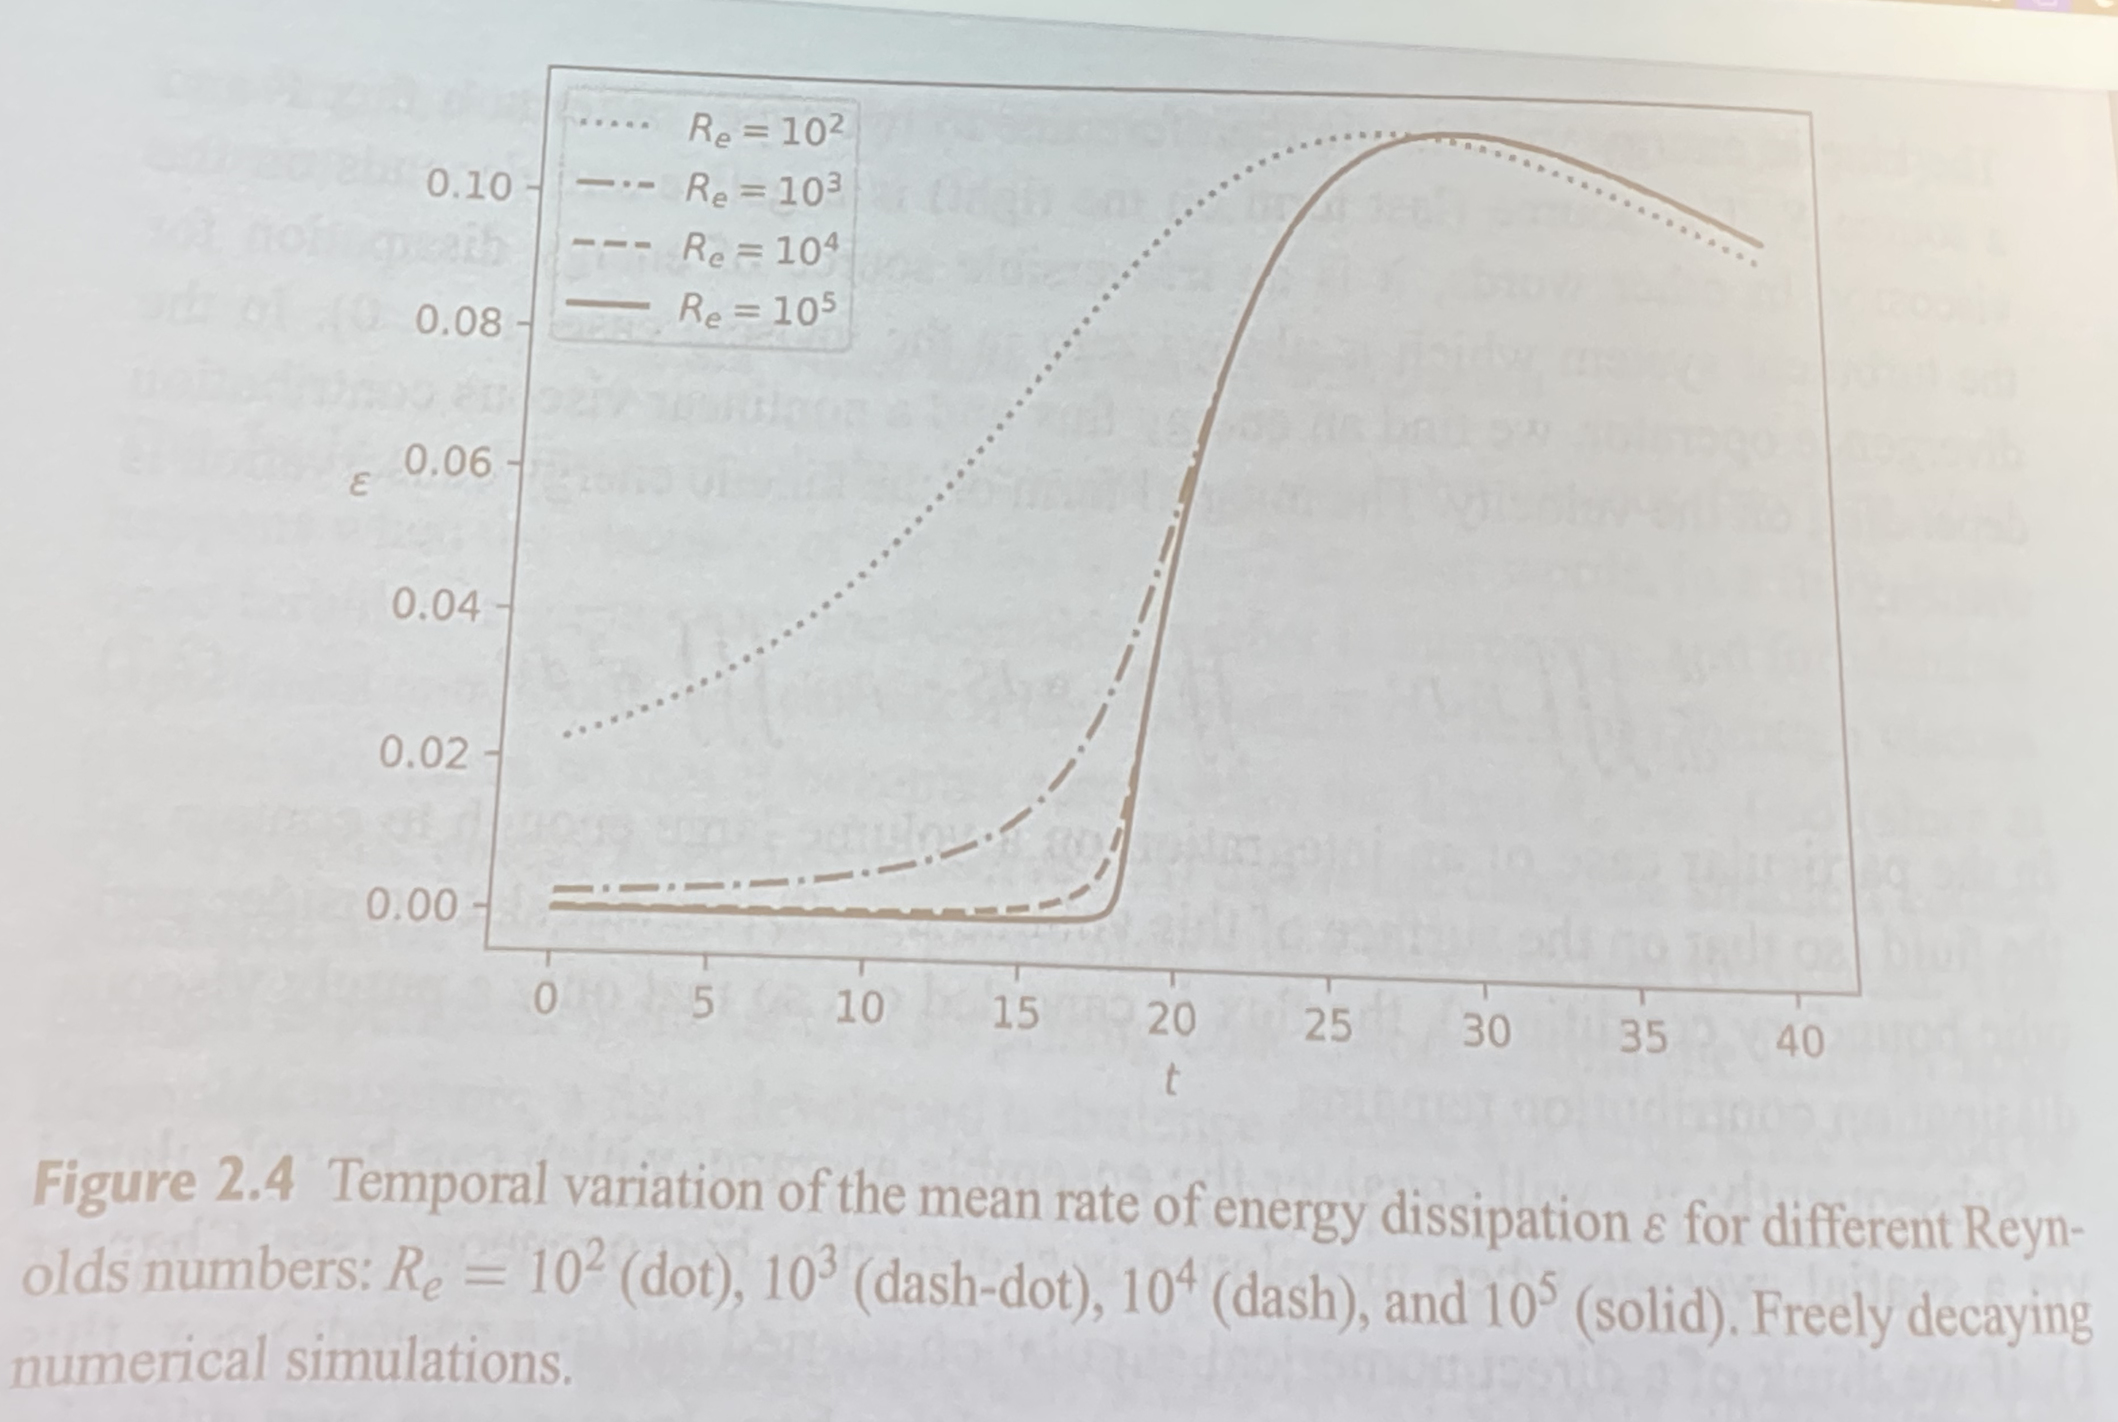
\includegraphics[scale=0.2]{Lectures/Images/lec13-eRecurves.png}
\end{center}

Next time, we will show that the enstrophy, together with the energy, are conserved quantities in two dimensions. Then, we will show that if we add in odd viscosity, that 3D flows look like 2D. Then, we will look at how odd viscosity changes the 2D turbulent cascade, and then also the 3D turbulent cascade as a result of quasi-2D-behaviour.